\section{Comparison within developmental stages}\label{sec:stages}
The pooled sample mixes developmental stages. Its dimension--error curve
combines variation within stages with differences between them. The next
experiment therefore asks whether fitting each stage separately gives lower
error or a different response to output dimension. It retains the same input
PC coordinate system and fitting settings, but evaluates new within-stage
cell samples. These fits completed at \stagegenerated.

\subsection{Samples, targets and fitting settings}
There are ten annotated stages. Labels beginning with E denote embryonic
stages; labels beginning with P denote postnatal stages. A new uniform
sample of 1,500 cells was drawn without replacement within each stage,
using the counts in Table~\ref{tab:stages}. There are 15,000 distinct cells
across the ten stage samples. This does not split the earlier pooled
1,500-cell sample, which would have left only 19 E12 cells.

\begin{table}[htbp]
\centering\begin{tabular}{lrr}\toprule
Stage & Available cells & Proposed sample \\ \midrule
E11 & 9,364 & 1,500 \\
E12 & 1,610 & 1,500 \\
E14 & 26,944 & 1,500 \\
E16 & 5,401 & 1,500 \\
E18 & 23,011 & 1,500 \\
P0 & 9,925 & 1,500 \\
P2 & 17,963 & 1,500 \\
P5 & 6,756 & 1,500 \\
P8 & 11,727 & 1,500 \\
P14 & 8,103 & 1,500 \\
\bottomrule\end{tabular}

\caption{Available cells in the 120,804-cell input and the sample used per
developmental stage. Counts are cells, not biological replicates. Equal
sample sizes keep the number of evaluation pairs and landmark fraction
fixed; no stage is excluded.}
\label{tab:stages}
\end{table}

Targets use the same full-population 1,814-PC coordinates as
Section~\ref{sec:dimension}, without refitting the input PCs, whitening,
or stage-specific standardization. The global 99.002235-percent variance
retention does not imply that this exact fraction holds within each stage.
For local-neighbor selection only, each stage preparation uses a centered,
unscaled PCA retaining at least 90 percent of its sampled variance.
Target distances always use all 1,814 input PCs.

Every stage has one preparation shared across dimensions
$d\in\{3,4,5,10,20,25,50\}$: 200 internally selected distance-proportional
landmarks, symmetric union-of-ten-nearest-neighbor local interactions, and
regional endpoint counts. Each fit uses the SGD backend, one start,
inverse-squared distance weights, and 100 epochs on a 100-epoch Zheng
schedule with $\epsilon=0.1$. There is no edge-KK refinement or post-fit
scale adjustment. Sampling seeds are 2026102001--2026102010 and preparation
seeds are 20261101--20261110 in the table's stage order.
Initialization and fitting use seed 20190619 throughout. Within each
stage, nested Gaussian columns and the earlier initial-scale formula
match the pooled dimension experiment's initialization rule. Different
stage distances imply different fitted starting scales and weight-dependent
numeric learning rates.

All 70 attempted fits completed 100 epochs. None failed, were skipped, or
were excluded. A replenished queue shared ten single-threaded worker slots
between preparation and fitting. The pipeline, from input checks and
subsetting through the final fit, took \stageelapsedminutes\ minutes;
this excludes independent validation and report rendering. Peak sampled
aggregate resident memory was \stagepeakmemory\ GiB under the 50 GiB
watchdog threshold. The per-task native workspace allowance was 4 GiB.
The full-population run's pause and checkpoint records were unchanged.

\subsection{Evaluation and numerical checks}
For each stage $s$, the score $R_s(d)$ is Equation~\eqref{eq:full} evaluated
on all $M=1,124,250$ unordered pairs in its fixed 1,500-cell sample.
The sparse proxy remains separate. There is no evaluation-pair sampling,
and the same pairs are used across dimensions within a stage. Different
stages, and the pooled reference, necessarily evaluate different cell pairs.

A separate report script recomputed every final all-pairs score and proxy
using distances obtained from Gram matrices, rather than the fitting
runner's distance-vector calculation. All 70 scores agreed within
$10^{-8}$ percentage points. The script also checked preparation identities,
completed epochs, seeds, terminal-coordinate units, and the fitted/remaining
pair decomposition of Equation~\eqref{eq:partition}. Ten-epoch score histories
and final restartable states are retained for every fit.

Table~\ref{tab:stage-results} gives every tested stage and dimension.
Figure~\ref{fig:stage-curves} uses common axes, so the shape and level of
each stage curve can be compared with the pooled reference. These are
individual fits. One cell sample, one preparation, and one start per stage
do not support uncertainty intervals for stage rankings.

\begin{table}[htbp]
\centering\small\begin{tabular}{lrrrrrrr}\toprule
Stage & 3D & 4D & 5D & 10D & 20D & 25D & 50D \\ \midrule
E11 & 33.12 & 27.72 & 24.21 & 15.87 & 10.63 & 9.18 & 6.25 \\
E12 & 31.00 & 26.16 & 22.94 & 15.14 & 10.07 & 8.94 & 6.10 \\
E14 & 31.22 & 26.24 & 22.85 & 15.32 & 10.49 & 9.18 & 6.26 \\
E16 & 31.47 & 26.63 & 23.14 & 15.45 & 10.47 & 9.18 & 6.38 \\
E18 & 30.91 & 25.93 & 23.00 & 15.05 & 10.60 & 9.37 & 6.44 \\
P0 & 31.20 & 26.30 & 22.88 & 15.32 & 10.53 & 9.28 & 6.38 \\
P2 & 30.63 & 25.76 & 22.46 & 15.07 & 10.26 & 9.19 & 6.29 \\
P5 & 30.93 & 26.00 & 22.52 & 15.17 & 10.43 & 9.38 & 6.87 \\
P8 & 32.11 & 27.28 & 23.74 & 15.94 & 11.03 & 9.87 & 6.98 \\
P14 & 31.86 & 26.90 & 23.52 & 16.00 & 10.96 & 9.79 & 6.73 \\
\midrule
Pooled & 30.16 & 25.48 & 22.25 & 14.85 & 10.00 & 8.99 & 6.24 \\
\bottomrule\end{tabular}

\caption{All-pairs RMS relative distance error (percent) after 100 SGD
epochs. Columns are output dimensions; rows are independent stage samples.
The pooled row repeats the existing mixed-stage sample at the same
dimensions. All targets use the same global 1,814-PC coordinate system,
but each row has its own cells and target distances. Lower is better for
that sample's reconstruction criterion; these are not matched-cell
comparisons or replicate means.}
\label{tab:stage-results}
\end{table}
\FloatBarrier

\begin{figure}[p]
\centering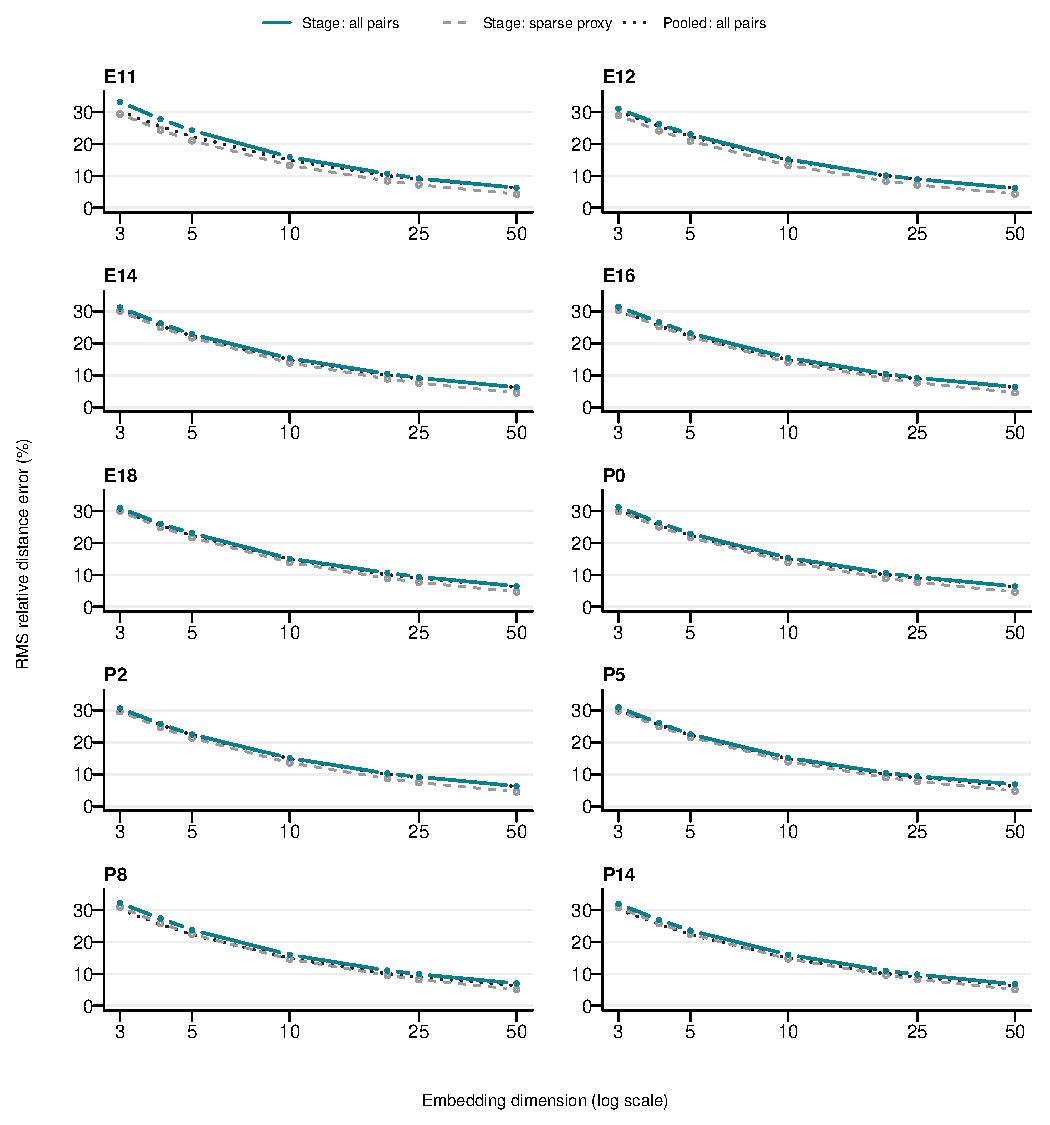
\includegraphics[width=\linewidth]{stage-error-curves.pdf}
\caption{Dimension--error curves for the ten stage samples, each containing
1,500 cells. Filled teal points show $R_s(d)$; open gray points show the
stage's sparse proxy; the dotted black line repeats the pooled all-pairs
curve. All seven tested dimensions are plotted on a logarithmic horizontal
axis; only selected ticks are labeled for readability. Vertical limits
are identical across panels. Connecting segments guide the eye. No
confidence bands are available from one fit per stage and dimension.}
\label{fig:stage-curves}
\end{figure}
\FloatBarrier

Error decreases with dimension in every stage, but stage restriction does
not produce the hoped-for reduction in achieved 3D error. Stage-specific
3D scores range from 30.626 percent (P2) to 33.116 percent (E11), compared
with 30.164 percent for the pooled sample. At 20D the range is
10.069--11.025 percent, compared with 10.000 percent pooled; at 50D it is
6.096--6.983 percent, compared with 6.242 percent pooled.
The broad dimension response is similar across stages, with modest
differences in level. These observations concern achieved reconstruction
error under this procedure, not minimum attainable error or biological
intrinsic dimension.

To make the small differences visible, define
\begin{equation}
\Delta_s(d)=R_s(d)-R_{\rm pooled}(d).
\end{equation}
Here $R_{\rm pooled}(d)$ is the earlier mixed-stage sample's all-pairs RMS
percentage at dimension $d$. Thus $\Delta_s$ has units of percentage
points: positive means higher stage-specific error, negative means lower.
This is a descriptive reference contrast, not a paired estimate on identical
cells. Figure~\ref{fig:stage-contrasts} displays all 70 contrasts.

\begin{figure}[p]
\centering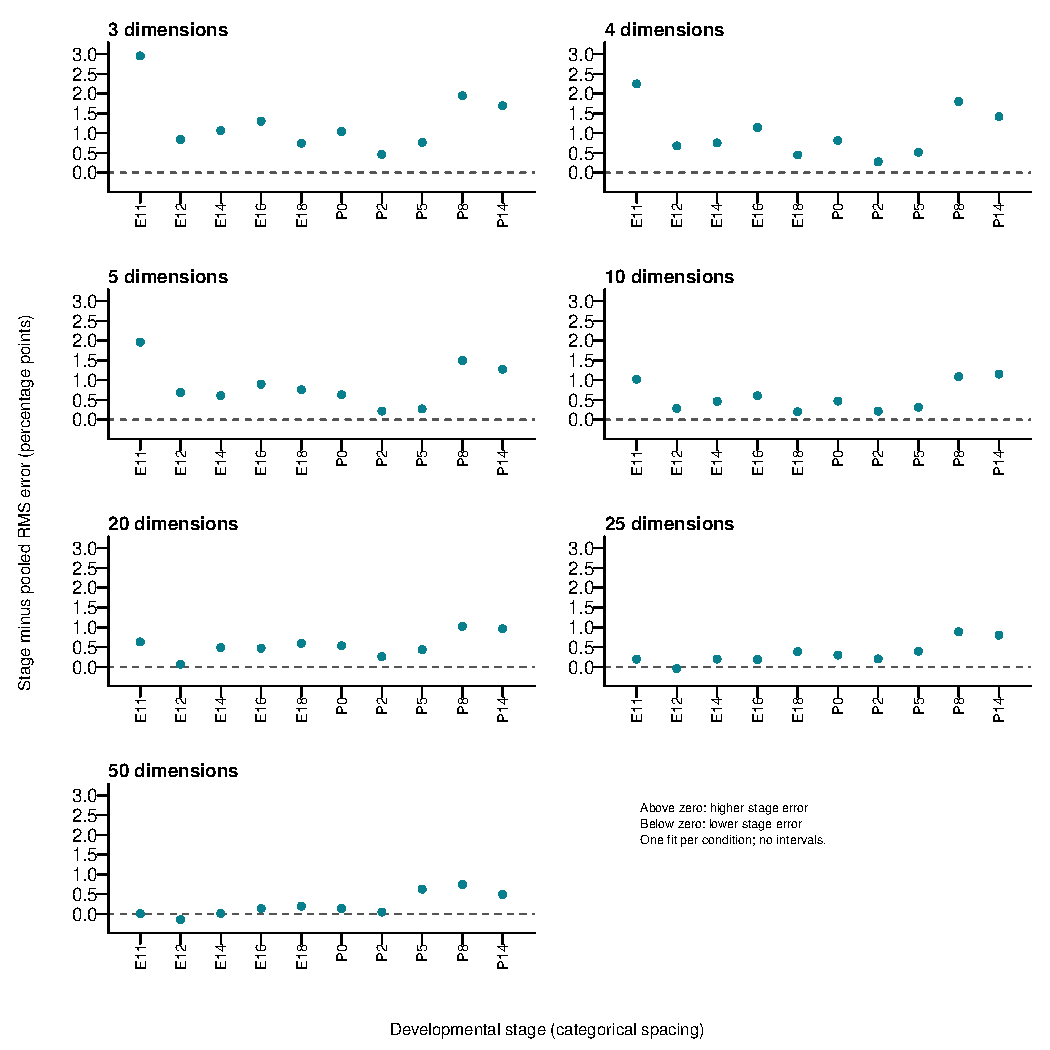
\includegraphics[width=\linewidth]{stage-pooled-differences.pdf}
\caption{Stage-minus-pooled RMS error differences $\Delta_s(d)$ in
percentage points, with one panel per output dimension. The dashed zero
line indicates equal scores. Each point is one fit; there are no replicate
intervals or significance tests. Stage positions are categorical and
equally spaced, not a numerical age axis. Identical vertical limits make
effect sizes comparable across dimensions.}
\label{fig:stage-contrasts}
\end{figure}

Sixty-eight of the 70 stage--dimension combinations have higher error than
the corresponding pooled fit. The two exceptions are E12 at 25D
(8.942 versus 8.987 percent) and 50D (6.096 versus 6.242 percent).
Those advantages are only 0.045 and 0.146 percentage points. They should
not be interpreted as robust stage differences from a single run.
The sparse proxy is below all-pairs error in every fit, by 0.889--3.764
percentage points, so it would understate the requested reconstruction
error if reported in its place.

\subsection{Geometry and interpretation}
The preparatory search projections retain 453--583 PCs. Mean ten-neighbor
retention against search in all 1,814 PCs ranges from 83.1 to 90.1 percent.
As above, this is
$1500^{-1}\sum_i |N_i^{1814}\cap N_i^{\rm search}|/10$,
where each set contains the ten nearest other sampled cells.
It measures neighbor-selection changes, not the quality of the fitted
embedding. Table~\ref{tab:stage-preparation} reports these diagnostics
alongside the median target distance, namely the median of all
1,124,250 values $d_{ij}$ in the stage sample.

\begin{table}[htbp]
\centering\small\begin{tabular}{lrrr}\toprule
Stage & Search PCs & Neighbor retention (\%) & Median target distance \\ \midrule
E11 & 454 & 88.7 & 9.15 \\
E12 & 472 & 90.1 & 7.86 \\
E14 & 459 & 86.6 & 10.63 \\
E16 & 453 & 83.1 & 11.50 \\
E18 & 513 & 89.0 & 11.59 \\
P0 & 493 & 88.6 & 11.29 \\
P2 & 491 & 88.5 & 12.01 \\
P5 & 541 & 86.2 & 14.72 \\
P8 & 578 & 88.6 & 16.51 \\
P14 & 583 & 84.0 & 16.42 \\
\bottomrule\end{tabular}

\caption{Stage-specific preparation diagnostics. Search PCs is the number
of coordinates used only to select local neighbors. Neighbor retention
is the mean set-intersection fraction expressed as a percentage. Median
target distance is in the unscaled global PC coordinate units and
summarizes the within-stage distance distribution; it is not an error.
No target distances are replaced by search-projection distances.}
\label{tab:stage-preparation}
\end{table}
\FloatBarrier

Median target distances range from 7.86 in E12 to 16.51 in P8, despite
using the same coordinate system. Relative error divides each pair's
residual by its own target distance. Consequently the pooled and
within-stage percentages are not interchangeable absolute-error measures.
A lower pooled score does not establish that the mixed biological
population is simpler.

The experiment does not support the expectation that fitting age-restricted
samples alone will substantially lower the observed 3D relative error.
It does not show that developmental structure is absent. Residual
within-stage variation, cell-type composition, noise, the sparse
approximation and finite optimization remain possible contributors.
Different stage preparations and random samples also prevent attributing
the differences to age alone. Multiple starts and independent cell
subsamples are needed before ranking stages reliably; matched landmark
and optimization sensitivity tests would address the remaining algorithmic
uncertainty. The full 120,804-cell experiment remains paused.
